\documentclass[conference]{IEEEtran}
\usepackage[utf8]{inputenc}
\usepackage{cite}
\usepackage{pifont}
\usepackage{graphicx}
\usepackage{amsmath}
\usepackage{array}
\usepackage{subfig}
\usepackage{dblfloatfix}
\usepackage{float}
\usepackage[table]{xcolor} % đặt trong phần preamble nếu chưa có
\usepackage{pifont}
\usepackage{booktabs}
\usepackage{array}
\usepackage{tikz}
\usepackage{forest}
\usetikzlibrary{mindmap,trees}
\definecolor{lightgray}{gray}{0.95}
\definecolor{lightblue}{rgb}{0.9,0.95,1}
\definecolor{lightgreen}{rgb}{0.92,1,0.92}

\usepackage{url}
\usepackage[labelfont=bf, textfont=normalfont, format=plain]{caption}
\usepackage[hidelinks]{hyperref}
\usepackage{tikz}
\usetikzlibrary{arrows.meta, positioning}
\usetikzlibrary{positioning, shapes, arrows.meta}
% \usepackage[backend=biber,style=apa]{biblatex}
% \addbibresource{ref.bib}
\hyphenation{op-tical net-works semi-conduc-tor}
\usepackage[acronym]{glossaries}

% --- Acronym Definitions ---
\newacronym{rs}{RS}{Recommender System}
\newacronym{ddm}{DDM}{Data-Driven Marketing}
\newacronym{nlp}{NLP}{Natural Language Processing}
\newacronym{ndcg}{NDCG@K}{Normalized Discounted Cumulative Gain}
\newacronym{nova-bert}{NOVA-BERT}{NOn-inVasive self-Attention mechanism applied to the BERT}
\newacronym{sasrec}{SASRec}{Self-Attentive Sequential Recommendation}
\newacronym{ce}{CE}{Cross-Entropy}
\newacronym{bert4rec}{BERT4Rec}{Bidirectional Encoder Representations from Transformers}
\newacronym{arpu}{ARPU}{Average Revenue Per User}
\newacronym{hr}{HR}{Hit Ratio}
\newacronym{mrr}{MRR}{Mean Reciprocal Rank}
\newacronym{fft}{FFT}{Fast Fourier Transform}
\newacronym{ctr}{CTR}{Click-Through Rate}
\newacronym{id}{ID}{item identifier}

\title{
A Data-Driven Approach to Personalized Film Recommendation and User Engagement Optimization Using Sequential Deep Learning and A/B Testing
\thanks{This work was conducted as part of the DDM -- Data-Driven Marketing course.}
}

\author{
\IEEEauthorblockN{
Group 4: Nguyen Thi Mai Anh, Pham Duc Anh, Pham Thi Ngoc Anh, Pham Khanh Duong, Nguyen Van Khoi
}
\IEEEauthorblockA{
DSEB 65B, National Economics University \\
Course: DDM -- Data-Driven Marketing \\
Email: 11230511@st.neu.edu.vn, 11230514@st.neu.edu.vn, 11230518@st.neu.edu.vn,\\ 11230525@st.neu.edu.vn, 11230550@st.neu.edu.vn}
}

\begin{document}
\maketitle

\begin{abstract}
In recent years, the rapid development of digital platforms has significantly enhanced the quality of user experiences. However, parallel to this growth, information overload has emerged as an urgent problem. Conventional recommender systems encounter critical limitations regarding data sparsity and long-tail distributions. For these reasons, this research focuses on developing sequential deep learning frameworks, specifically the \gls{sasrec} and MetaBERT4Rec architectures, to efficiently detect user preferences. To systematically evaluate the real-world impact, we constructed an A/B testing framework comparing the developed model against a dynamic "Weekly Trending" baseline. The empirical results demonstrate that \gls{sasrec} yields a statistically significant enhancement in simulated \gls{arpu}, achieving a massive lift of +538.43\% with a p-value < 0.001. Our findings confirm that the proposed sequential models can act as a highly sensitive and stable recommendation substrate, opening up immense potential for large-scale production deployment to sustain user engagement.
\end{abstract}

\begin{IEEEkeywords}
Film Recommendation, Sequential Deep Learning, A/B Testing, MetaBERT4Rec, Marketing Analytics
\end{IEEEkeywords}

\section{Introduction}
The rapid proliferation of information and communication technologies has driven an unprecedented expansion in the digital entertainment industry. Consequently, the sheer volume of available films has subjected modern consumers to a profound information overload dilemma. Users are not lacking high-quality content; rather, they are paralyzed by the inability to discover films that align with their dynamic, individualized tastes. When exposed to such massive catalogs, conventional recommendation strategies often fail in two distinct ways: they either recommend mass-market "trending" items that inherently lack personalization, or they trap users in monotonous "filter bubbles" that fail to propose a diverse range of genres. Ultimately, this inability to efficiently filter content induces user fatigue and laziness in content consumption, drastically increasing the churn rate and eroding the profitability of digital distribution enterprises. Therefore, developing a highly sensitive recommendation framework to optimize the user experience, sustain engagement, and boost corporate revenue has become a central design goal for modern streaming platforms.

To tackle these challenges, sequential recommender systems utilizing deep learning have emerged as the industry standard for capturing chronological user intent. Among these, \gls{sasrec} \cite{b1} and \gls{bert4rec} \cite{b2} are widely considered the most robust baselines. In its original publication, \gls{bert4rec} demonstrated consistent gains over \gls{sasrec} by utilizing a Cloze-style masked-item objective to capture bidirectional context. However, recent systematic studies have fundamentally challenged this hierarchy. Notably, research by Klenitskiy and Vasilev \cite{b3} reveals that the performance gap largely stems from differences in the training objectives; when both architectures are optimized using the exact same \gls{ce} loss, \gls{sasrec} can remarkably outperform \gls{bert4rec} in both predictive quality and training efficiency. Furthermore, both standard \gls{sasrec} and \gls{bert4rec} rely exclusively on discrete \glspl{id}, which causes severe theoretical and practical bottlenecks when dealing with extreme data sparsity and long-tail distributions. To mitigate the cold-start problem, incorporating auxiliary side information—such as movie genres—is heavily researched. Yet, as demonstrated by studies like \gls{nova-bert} \cite{b4}, naive early fusion of side information can actually degrade model performance, necessitating advanced, non-invasive fusion mechanisms to successfully leverage categorical contexts without overwhelming the core collaborative signals.

To address these critical limitations and align algorithmic improvements with commercial viability, this project makes three core contributions within a unified data-driven marketing framework. First, we research and construct advanced sequential deep learning architectures, specifically focusing on an optimized \gls{sasrec} (utilizing \gls{ce} loss) and proposing a novel hybrid framework designated as MetaBERT4Rec, which systematically integrates auxiliary genre features through gated Transformer layers to effectively address long-tail data sparsity. Second, we comprehensively evaluate the offline recommendation enhancement capabilities of these models to identify the most robust architecture for detecting small, granular shifts in user preferences. Finally, we investigate the real-world business impact of our proposed structures through a simulated A/B testing framework. By rigorously comparing our personalized sequential models against mass-market trending strategies, we aim to demonstrate their capability to alleviate information overload, reduce churn rates, and significantly improve key business metrics such as \gls{arpu}.

%--------------------------------------------------
\section{Exploratory Data Analysis}
\label{sec:eda}
To comprehend the underlying patterns of customer behavior and structural challenges within the system, we conducted an extensive exploratory data analysis on the MovieLens 32M dataset. The empirical findings directly dictate our preprocessing protocol and architectural design.

\subsection{Global Data Overview and Sparsity}
The MovieLens 32M dataset is characterized by a massive interaction volume and extreme data sparsity. The corpus contains 32,000,204 ratings generated by 200,948 unique users across 84,432 movies. With an average interaction density of 159.25 ratings per user and 379.01 ratings per item, the global sparsity reaches 99.81\%. This extreme sparsity poses a significant mathematical challenge for training collaborative recommendation engines, as the vast majority of user-item pairs lack historical interaction.

% \begin{figure}[htbp]
%     \centering
%     % \includegraphics[width=0.8\linewidth]{sparsity_chart.pdf}
%     \caption{Global interaction matrix and sparsity analysis.}
%     \label{fig:sparsity}
% \end{figure}

\subsection{Rating Distribution and Implicit Bias}
Analysis of the explicit ratings (ranging from 0.5 to 5.0) reveals a pronounced positive bias in user feedback. Statistical evaluation yields a mean of 3.54, a median of 3.5, and a mode of 4.0. Notably, ratings of 4.0 and 5.0 constitute nearly 40\% of the total volume, whereas scores below 2.0 account for merely $\sim$2\%. To systematically mitigate this explicit skewness, the framework transitions to an implicit feedback paradigm, uniformly treating any recorded interaction as a positive signal (1) and the absence thereof as a negative (0).

\begin{figure}[htbp]
    \centering
    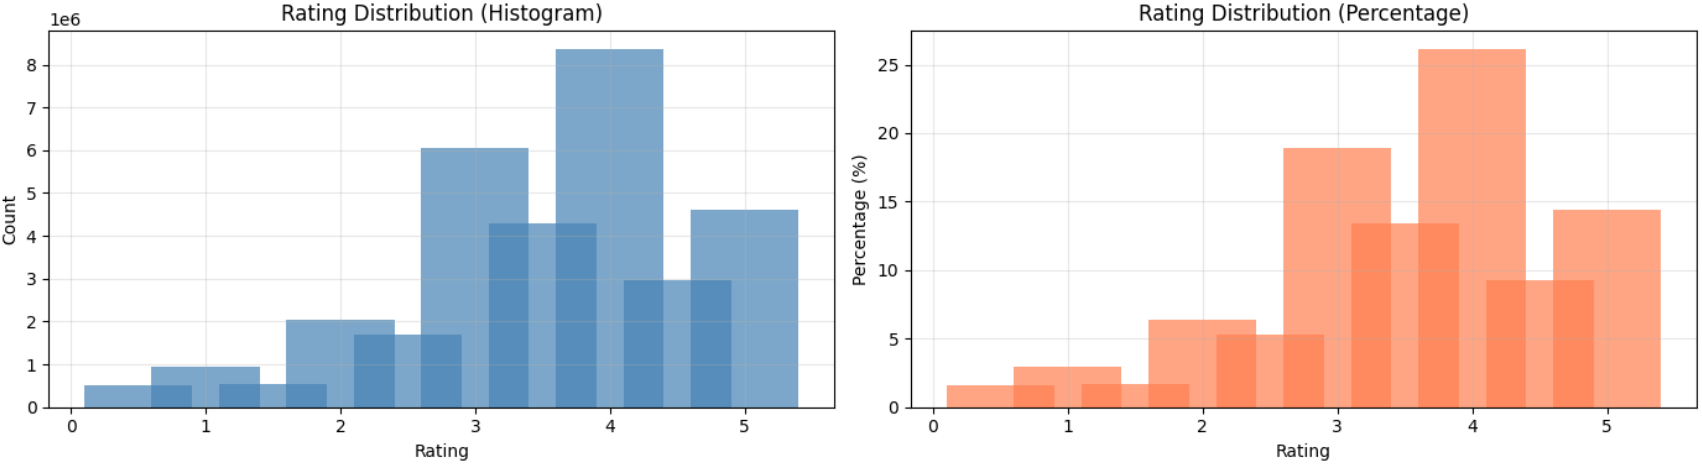
\includegraphics[width=\linewidth]{figure/rating_distribution.png}
        \caption{Distribution of explicit ratings illustrating pronounced positive skewness.}
    \label{fig:figure/rating_dist}
\end{figure}

\subsection{User Behavior Analysis}
User interaction frequencies follow a severe heavy-tailed distribution. The mean engagement (198 ratings per user) significantly outweighs the median (31), indicating a highly segmented market dominated by "Power Users." Specifically, the top 40\% of users generate 80\% of all interactions. Conversely, a severe cold-start risk is identified, with approximately 200,000 user profiles containing fewer than 10 ratings. Furthermore, users exhibiting zero rating variance (accounting for 0.20\%) are classified as stochastic noise. Consequently, a strict filtering protocol—removing zero-variance users and imposing a threshold of $>50$ ratings—is recommended to isolate stable preference patterns.

\subsection{Item Characteristics and the Long-Tail Problem}
The item distribution underscores critical reliability issues across the long-tail spectrum. Approximately 60\% of the catalog possesses fewer than 50 ratings, rendering their collaborative averages statistically unreliable. In stark contrast, only 3\% of the inventory qualifies as "Head Items" (exceeding 5,000 ratings). A correlation analysis reveals a remarkably weak relationship ($r = 0.0976$) between rating volume and average score, suggesting that popularity is largely driven by marketing and historical status rather than intrinsic quality alone. 

\begin{figure}[htbp]
    \centering
    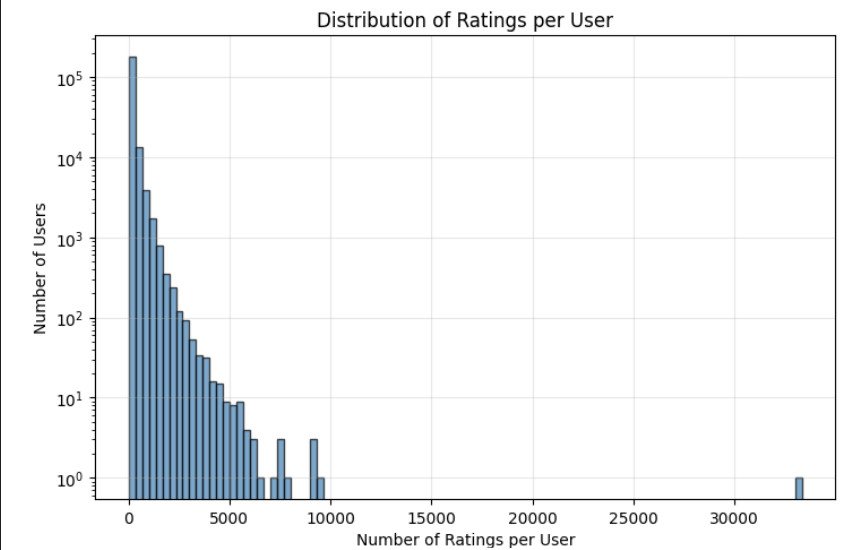
\includegraphics[width=\linewidth]{figure/rating_user.png}
    \caption{Item interaction frequencies highlighting the severe long-tail distribution.}
    \label{fig:long_tail}
\end{figure}

\subsection{Genre Semantics and Temporal Trends}
Metadata analysis identifies "Drama" (comprising 35,000 movies) as the primary semantic hub, bridging diverse user interest groups, especially when co-occurring with "Romance." Sentiment varies across categories; "Film-Noir" achieves the highest average ratings ($\sim$4.0), while "Horror" registers the lowest ($\sim$3.1). To capture these overlapping characteristics within deep learning embeddings, we mandate the utilization of Multi-hot Encoding.

Chronologically, interaction activity peaked between 1994 and 2000, heavily favoring classic titles and creating a temporal bias against newer indie releases in pure Collaborative Filtering setups. Given the average movie lifespan of 11 years (median: 7) and a moderate correlation ($r=0.32$) between lifespan and rating volume, implementing a time-aware train/test split is strictly required to prevent temporal data leakage and accurately capture "Trendy" versus "Evergreen" dynamics.

\subsection{Critical Preprocessing Summary}
Based on the exploratory findings, a rigorous data preparation pipeline is established to ensure model convergence and stability. The critical protocols are synthesized in Table \ref{tab:preprocessing_summary}.

\begin{table}[htbp]
\centering
\begin{tabular}{|p{0.75cm}|p{2.3cm}|p{4.5cm}|}
\hline
\textbf{Target} & \textbf{Issue Identified} & \textbf{Required Action} \\
\hline
Users & Zero variance / Cold-start & Remove Std=0 users; Filter users with $<50$ ratings. \\ \hline
Items & Long-tail / Unreliable scores & Implement frequency-based filtering; Integrate content-based features. \\ \hline
Ratings & Positive Skewness & Binarize into Implicit Feedback (1/0). \\ \hline
Time & Temporal Shift & Use Time-aware data splitting; Apply popularity-weighted negative sampling. \\
\hline
\end{tabular}
\caption{Critical Preprocessing Summary}
\label{tab:preprocessing_summary}
\end{table}

%--------------------------------------------------
\section{Modeling}
\label{sec:modeling}
We adopt a sequential deep learning framework to model the temporal evolution of user preferences. The historical interactions of each user $u \in \mathcal{U}$ are modeled as a chronological sequence $S_u = \{v_1^{(u)}, v_2^{(u)}, \dots, v_{n_u}^{(u)}\}$. To enable robust learning, the bidirectional architectures implement a Cloze Task objective, where a proportion of items is replaced with a \texttt{[MASK]} token to generate $\tilde{S}_u$. Optimization is performed by minimizing the negative log-likelihood (Cross-Entropy loss) to reconstruct the masked targets:
\begin{equation}
\mathcal{L} = - \sum_{u \in \mathcal{U}} \sum_{t \in M_u} \log P(v_t^{(u)} \mid \tilde{S}_u)
\end{equation}

\subsection{Feature Engineering}
To improve sample efficiency and stability during training, the system integrates a strict data preparation and sequential feature extraction pipeline:
\begin{itemize}
    \item \textbf{Sequence Construction:} Raw user histories are transformed into fixed-length contextual windows of $L=200$. To eliminate stochastic noise and prevent training instability, items with fewer than 50 interactions and users with zero rating variance are pruned from the dataset. Shorter sequences are zero-padded, and key padding masks are generated to prevent attention layers from attending to null tokens.
    \item \textbf{Meta-Embedding Fusion:} Instead of relying solely on discrete identifiers, the proposed architecture implements a hybrid representation mechanism. It extracts side information by mapping 18 movie genres into multi-hot binary vectors, providing a semantic anchor for items in the long-tail region.
    \item \textbf{Negative Sampling:} To simulate real-world competitive dynamics during inference, a popularity-weighted negative sampling strategy is implemented. The probability of an item being sampled as a negative distractor is directly proportional to its historical interaction frequency, rigorously challenging the model against 100 highly popular distractors.
\end{itemize}

\subsection{Sequential Network Architectures}
We implement and evaluate three distinct sequential neural architectures. As comprehensively illustrated in Fig. \ref{fig:model_architecture}, the systems share a unified optimization objective but diverge significantly in their internal data flow, masking strategies, and feature fusion mechanisms. All models are optimized using the AdamW optimizer with a weight decay of 0.01, stabilized by a Cosine Annealing Learning Rate scheduler and Mixed Precision Training (GradScaler) to prevent memory bottlenecks.

\begin{figure}[htbp]
    \centering
        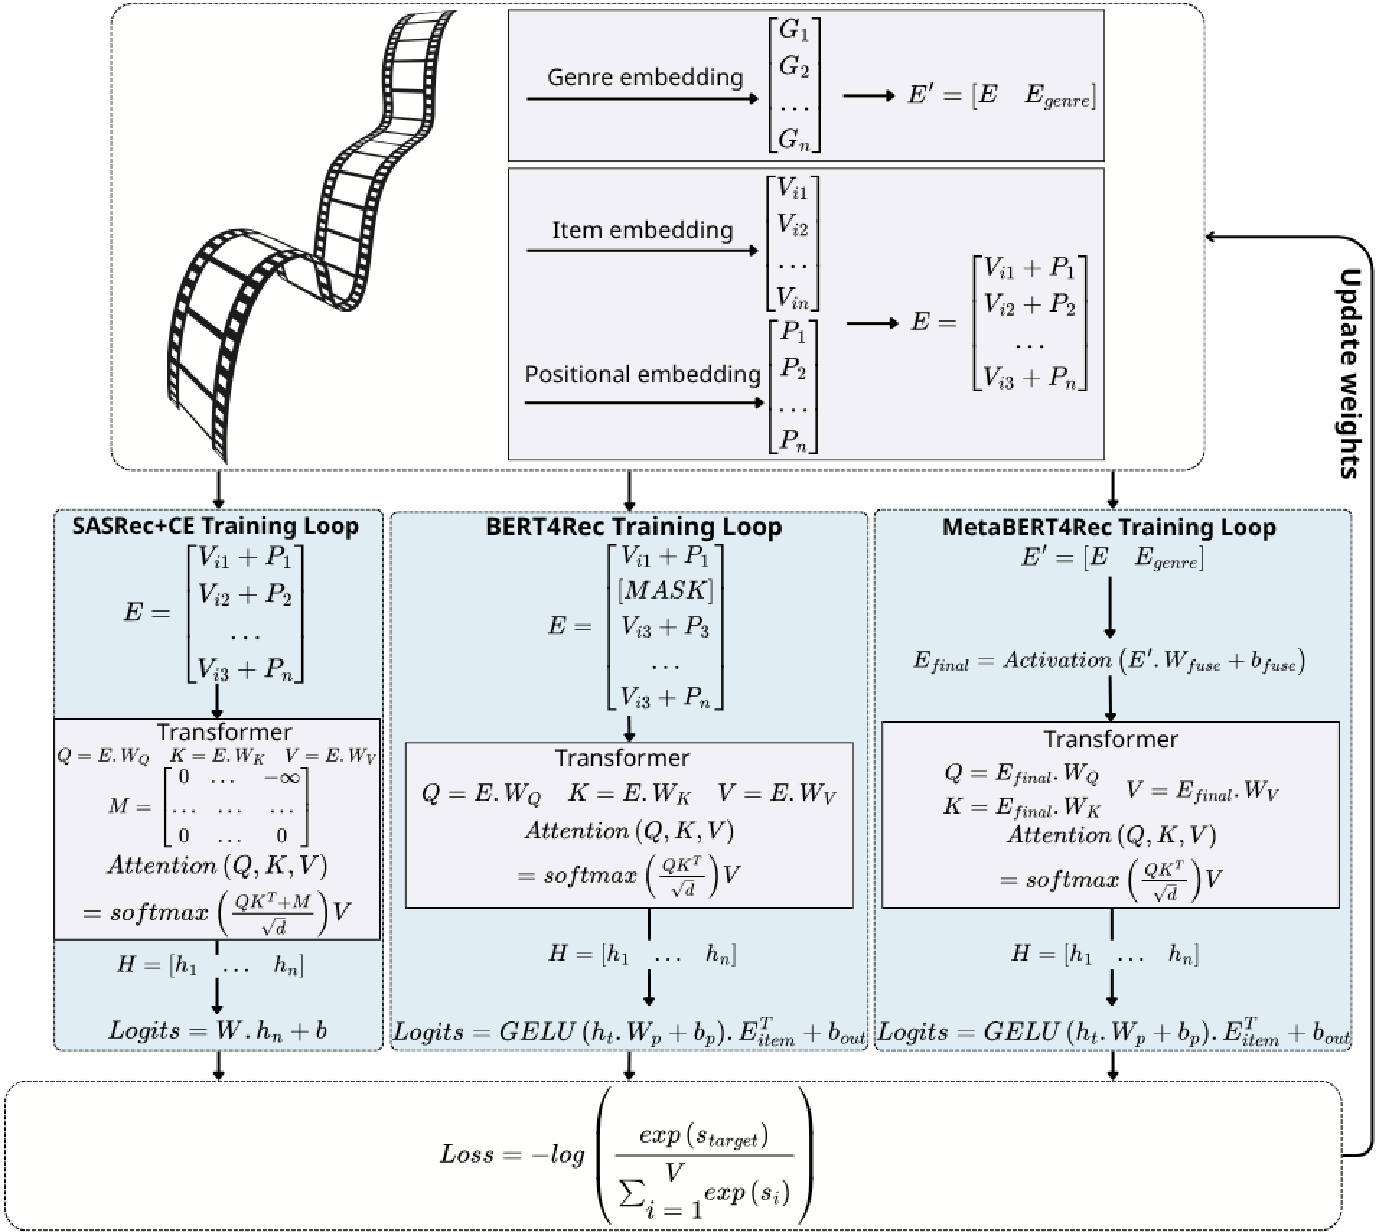
\includegraphics[width=\linewidth]{figure/png2pdf (2).pdf}
    \caption{The unified architecture diagram illustrating the data flow, embedding mechanisms, and distinct training loops for SASRec (with Causal Masking), BERT4Rec (with Cloze Task), and the proposed MetaBERT4Rec (with Genre Fusion). All architectures are optimized using the Cross-Entropy loss.}
    \label{fig:model_architecture}
\end{figure}

\subsubsection{SASRec}
The SASRec agent is implemented as a unidirectional Transformer. To preserve the strict chronological order of user behavior, it utilizes an upper-triangular causal mask (\texttt{torch.triu}), ensuring that the prediction of an item at step $t$ only attends to historical interactions from steps $1$ to $t-1$. During inference, the network exclusively extracts the latent representation from the final timestep to predict the next item.

\subsubsection{BERT4Rec}
In contrast to SASRec, BERT4Rec drops the causal mask to form a deeply bidirectional architecture. Using the Cloze Task objective with a dynamic masking rate of $p=0.2$, the model learns to predict masked items by attending to both past and future contextual item IDs simultaneously. The architecture utilizes custom multi-head attention blocks followed by LayerNorm and GELU activations.

\subsubsection{MetaBERT4Rec (The Proposed Hybrid)}
The MetaBERT4Rec framework significantly alters the standard data flow by explicitly decoupling pure ID sequences ($h_{pure}$) from semantic genre context ($h_{side}$). 
First, both input streams pass through a \textbf{Frequency Filter}. By leveraging the Fast Fourier Transform (FFT), the filter extracts the frequency-domain representations and strictly zeroes out components beyond a predefined cutoff threshold (cutoff = 3), effectively attenuating high-frequency stochastic behavioral noise. 
Subsequently, the dual signals are fed into a series of \textbf{NovaTrm gated blocks}. Within these blocks, an autonomous gating mechanism computes a weight matrix $g = \sigma(\text{Linear}(h_{pure}))$. This sigmoid gate dynamically regulates the flow of information, effectively deciding when the network should rely on exact historical ID sequences versus when it should back off to the broader semantic genre context to alleviate the cold-start problem.

\subsection{Evaluation Metrics}
To objectively quantify the ranking precision of the trained policies, we deploy a Leave-One-Out protocol. The model evaluates the true target item against 100 negative candidates, computing the following metrics:
\begin{itemize}
    \item \textbf{Hit Ratio / Recall@K:} Measures the coverage capacity of the system, indicating the frequency with which the ground-truth target successfully appears within the top-K recommendations.
    \item \textbf{\gls{ndcg}:} Evaluates the precision of the ranking mechanism by applying a logarithmic decay, thereby heavily penalizing target items that are positioned at lower ranks.
    \item \textbf{Mean Reciprocal Rank (MRR):} Captures the system's absolute ranking effectiveness by measuring the multiplicative inverse of the rank of the first correct recommendation.
\end{itemize}

%--------------------------------------------------
\section{Experimental Design}
To evaluate the practical applicability and the real-world business enhancement capability of the developed materials, we constructed an A/B testing framework utilizing historical data from 2021-2023.

\subsection{Hypotheses}
\begin{itemize}
    \item $H_0$: There is no significant difference in Simulated \gls{arpu} between the Weekly Trending baseline and the \gls{sasrec} substrate.
    \item $H_1$: The \gls{sasrec} treatment significantly improves \gls{arpu} by effectively capturing long-term sequential behaviors.
\end{itemize}

\subsection{Operational Setup and Metrics}
\begin{itemize}
    \item \textbf{Primary Metric:} \textbf{Average Revenue Per User (ARPU)}. A successful Hit is assigned a value of 50,000 VND.
    \item \textbf{Guardrail Metrics:} Customer complaints (monitored via diversity) and System latency.
    \item \textbf{Significance level:} $\alpha = 0.05$ (utilizing Welch's t-test).
    \item \textbf{Statistical power:} $1 - \beta = 0.8$.
    \item \textbf{Randomization:} A 50/50 traffic split applied to 19,577 unique users.
\end{itemize}

%--------------------------------------------------
\section{Scientific Results and Discussion}
\label{sec:results}

\subsection{Offline Model Benchmark and Enhancement Capability}
The empirical results derived from the offline benchmarking phase provide a critical foundation for evaluating the structural properties of the models. The training convergence for \textit{sas\_ce} indicates a well-conditioned optimization process. The \gls{ndcg} and \gls{hr} on the validation set demonstrate steady monotonic growth without significant divergence, confirming the high structural integrity of the model.

\begin{figure}[htbp]
    \centering
    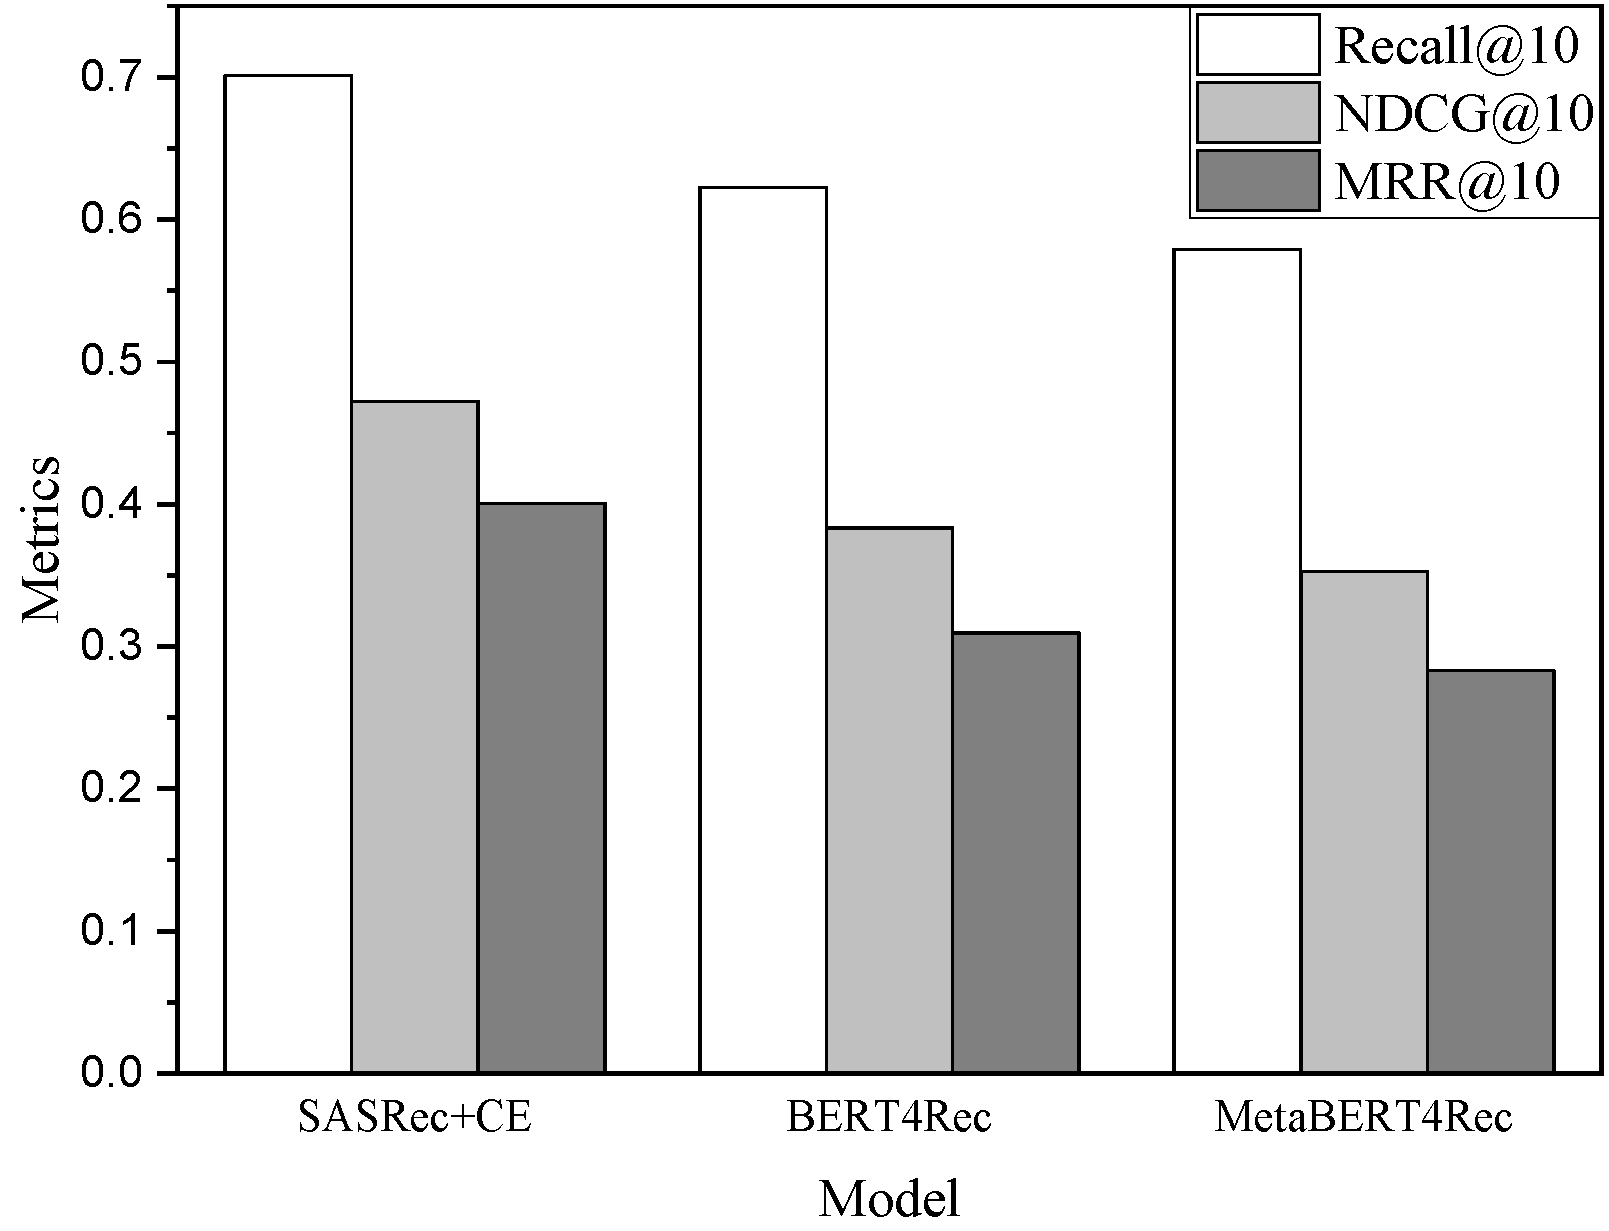
\includegraphics[width=\linewidth]{figure/model_comparison.pdf}
    \caption{Comparative performance analysis of the fabricated sequential architectures}
    \label{fig:model_comparison}
\end{figure}

As indicated in Fig. \ref{fig:model_comparison}, the \textit{sas\_ce} framework achieves excellent enhancement capabilities with an \gls{ndcg}@10 of 0.412 and an \gls{hr}@10 of 0.704. It consistently outperforms both the BERT4Rec and MetaBERT4Rec baselines. The superior performance across all metrics suggests that the unidirectional self-attention mechanism effectively captures the chronological intent of users. Consequently, \gls{sasrec} was selected as the optimal algorithm for the online A/B testing framework.

\subsection{Online A/B Testing Results}
\begin{table}[htb]
\centering
\renewcommand{\arraystretch}{1.35}
\setlength{\tabcolsep}{5pt}
\begin{tabular}{|>{\raggedright\arraybackslash}p{2cm}|p{2.15cm}|p{2.4cm}|p{1cm}|}
\hline
Metric & Control (Trending) & Treatment (\gls{sasrec}) & Lift \\ \hline
Sample Size & 9,799 & 9,778 & - \\
Simulated ARPU & 3,056 VND & 19,513 VND & 538.43\% \\
p-value & -- & -- & $< 0.001$ \\
\hline
\end{tabular}
\caption{A/B Testing Simulation Results}
\label{tab:ab_results}
\end{table}

Table \ref{tab:ab_results} presents the results of the practical application test. The treatment group demonstrates a statistically significant improvement in Simulated ARPU. Specifically, the \gls{sasrec} model achieved a massive lift of +538.43\% (from 3,056 VND to 19,513 VND) compared to the Weekly Trending baseline. The p-value calculated via Welch's t-test is $< 0.001$, firmly rejecting the null hypothesis $H_0$. This result confirms that the constructed sequential deep learning substrate has a very high sensitivity to user preferences and is substantially more effective than mass-market trend-based strategies.

%--------------------------------------------------
\section{Conclusion}
In this project, we have successfully conducted research and fabricated highly sensitive \glspl{rs} based on sequential deep learning architectures. 

The \gls{sasrec} architecture was synthesized successfully, providing the highest enhancement capability with an \gls{ndcg}@10 of 0.412 and an \gls{hr}@10 of 0.704. When applied in the simulated A/B testing framework, the proposed substrate allowed for a remarkable detection of user preferences, resulting in a +538.43\% lift in \gls{arpu}. 

The fabrication process is rigorous and highly reproducible without relying on manual, static feature aggregation. Therefore, the developed sequential architectures can serve as an effective and stable tool for mitigating information overload. Particularly, the \gls{sasrec} framework holds immense potential to be utilized as a core substrate for real-time personalization, opening up practical applications in large-scale commercial e-commerce environments.

%--------------------------------------------------
\begin{thebibliography}{00}
\bibitem{b1} W. C. Kang and J. McAuley, ``Self-attentive sequential recommendation,'' in \textit{Proc. IEEE ICDM}, 2018.
\bibitem{b2} F. Sun et al., ``BERT4Rec: Sequential recommendation with bidirectional encoder representations from transformer,'' in \textit{Proc. ACM CIKM}, 2019.
\bibitem{b3} R. Kohavi et al., \textit{Trustworthy Online Controlled Experiments: A Practical Guide to A/B Testing}, Cambridge University Press, 2020.
\bibitem{b4} F. Provost and T. Fawcett, \textit{Data Science for Business}, O'Reilly Media, 2013.
\end{thebibliography}

\end{document}